\documentclass{article}

\usepackage{graphicx}
\usepackage{tikz}
\usepackage{tikzsymbols}
\usetikzlibrary{calc,patterns,shapes.geometric}
\pagestyle{empty}
\usepackage[margin=0pt]{geometry}
\geometry{papersize={14in,12in}}

\def\centerarc[#1](#2)(#3:#4:#5){\draw[#1] ($(#2)+({#5*cos(#3)},{#5*sin(#3)})$) arc (#3:#4:#5);}

\begin{document}
	\begin{figure}
		\centering
		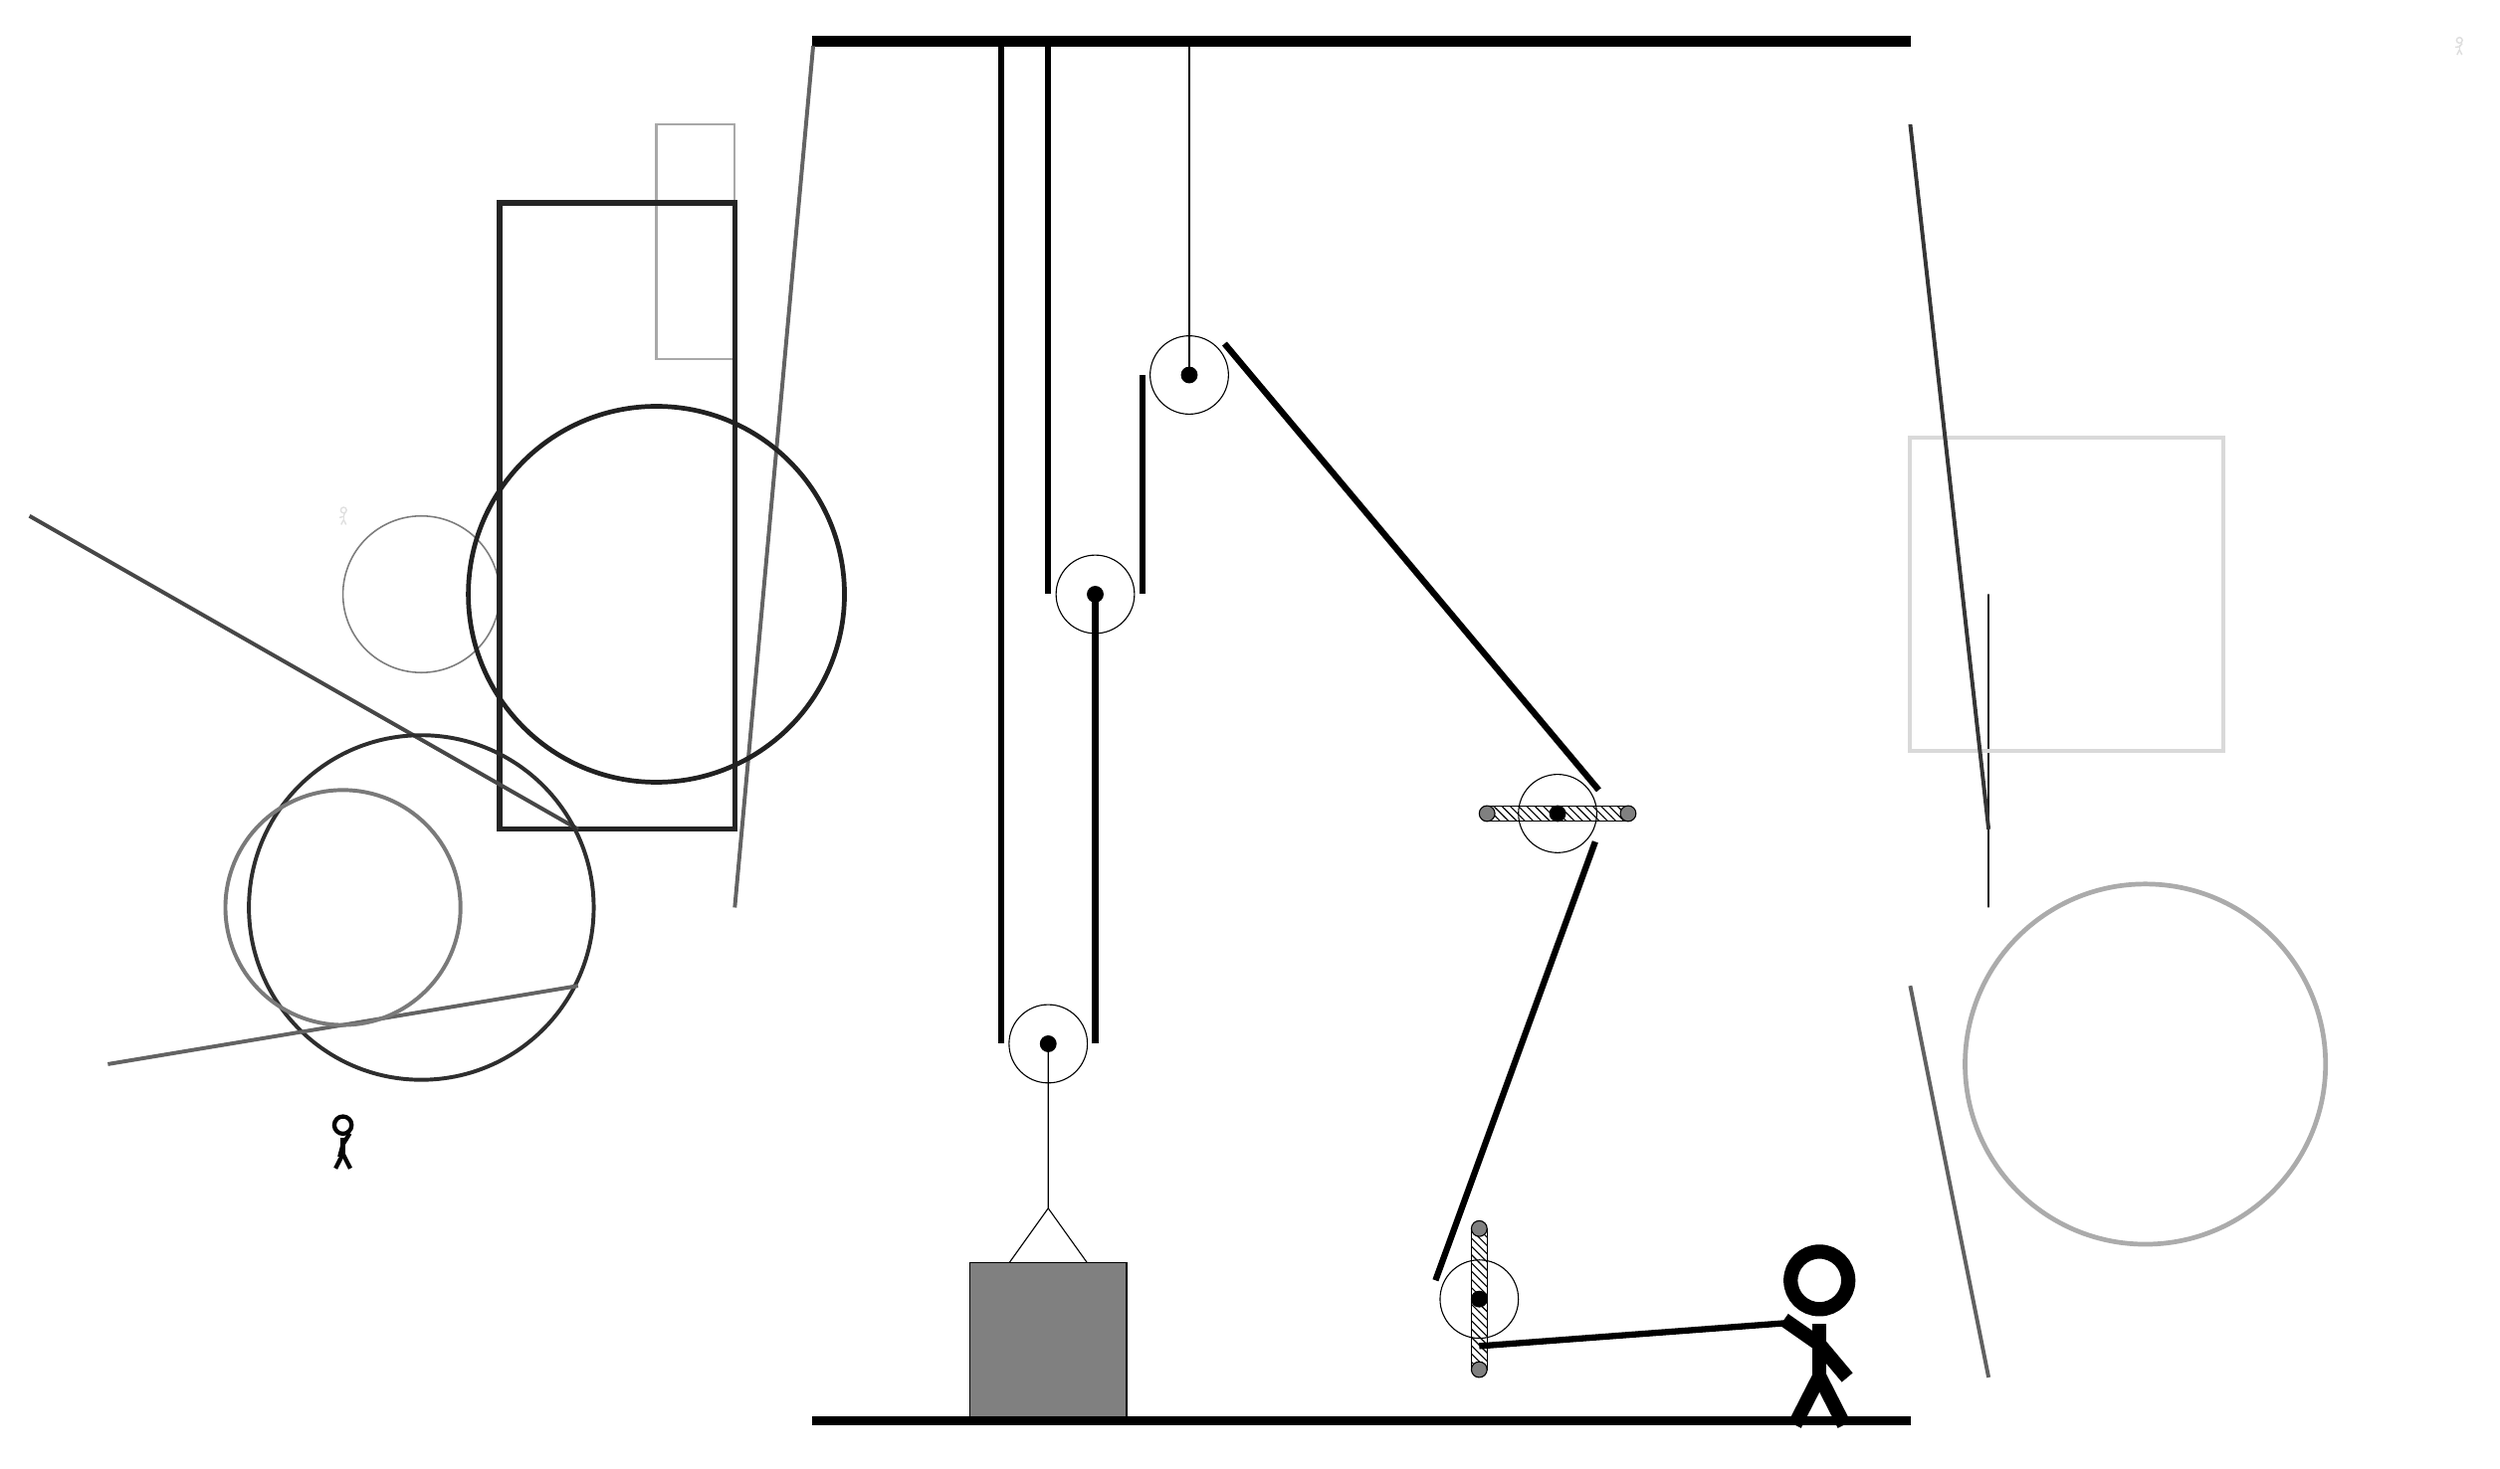
\begin{tikzpicture}
			%%%%% START %%%%%
			
			\draw[fill=black] (-2, 14) rectangle (12, 14.125);
			
			\draw [line width=0.6mm, color=black!33](15, 1) circle (2.3);
			
			\draw[line width=0.3mm, color=black!91] (13, 7) rectangle (13, 3);
			\draw[line width=0.5mm, color=black!61](-3, 3) -- (-2, 14);
			\draw[line width=0.5mm, color=black!15] (12, 5) rectangle (16, 9);
			\draw [line width=0.2mm, color=black!51](-7, 7) circle (1.0);
			\draw[line width=0.3mm, color=black!34] (-4, 13) rectangle (-3, 10);
			\draw[line width=0.7mm, color=black!86] (-3, 4) rectangle (-6, 12);
			\node[line width=0.2mm, color=black!99] at (-8, 0) {\Strichmaxerl[3][75][58]};
			\node[line width=0.5mm, color=black!12] at (-8, 8) {\Strichmaxerl[1][13][75]};
			\draw[line width=0.5mm, color=black!72](-5, 4) -- (-12, 8);
			
			\draw [line width=0.5mm, color=black!82](-7, 3) circle (2.2);
			\draw[line width=0.5mm, color=black!62](13, -3) -- (12, 2);
			\draw[line width=0.5mm, color=black!61](-5, 2) -- (-11, 1);
			
			\draw[line width=0.5mm, color=black!79](13, 4) -- (12, 13);
			\draw [line width=0.6mm, color=black!87](-4, 7) circle (2.4);
			\draw [line width=0.6mm, color=black!83](-5, 13) circle (0.0);
			
			\draw [line width=0.5mm, color=black!52](-8, 3) circle (1.5);
			
			\node[line width=0.7mm, color=black!13] at (19, 14) {\Strichmaxerl[1][7][50]};
			
			\draw (1, 1.26) circle (0.5);
			\draw[fill=black] (1, 1.26) circle (0.1);
			
			\draw (1.6, 7.0) circle (0.5);
			\draw[fill=black] (1.6, 7.0) circle (0.1);
			
			\draw (2.8, 9.8) circle (0.5);
			\draw[fill=black] (2.8, 9.8) circle (0.1);
			\draw[thick] (2.8, 9.8) -- (2.8, 14);
			
			\draw (6.5, -2) circle (0.5);
			\draw[fill=black] (6.5, -2) circle (0.1);
			\draw[pattern=north west lines, pattern color=black] (6.4, -1.1) rectangle (6.6, -2.9);
			\draw[fill=black!50] (6.5, -1.1) circle (0.1);
			\draw[fill=black!50] (6.5, -2.9) circle (0.1);
			
			\draw (7.5, 4.2) circle (0.5);
			\draw[fill=black] (7.5, 4.2) circle (0.1);
			\draw[pattern=north west lines, pattern color=black] (6.6, 4.3) rectangle (8.4, 4.1);
			\draw[fill=black!50] (6.6, 4.2) circle (0.1);
			\draw[fill=black!50] (8.4, 4.2) circle (0.1);
			
			\draw (1, 1.26) -- (1, -0.84) -- (0.5, -1.54) -- (1.5, -1.54) -- (1, -0.84);
			\draw[fill=black!50] (0, -1.54) rectangle (2, -3.54);
			
			\draw[line width=0.8mm] (0.4, 14) -- (0.4, 1.26);
			\centerarc[line width=0.8mm](1, 1.26)(180:360:0.6);
			\draw[line width=0.8mm](1.6, 1.26) -- (1.6, 7.0);
			\draw[line width=0.8mm] (1.0, 14) -- (1.0, 7.0);
			\centerarc[line width=0.8mm](1.6, 7.0)(180:360:0.6);
			\draw[line width=0.8mm](2.2, 7.0) -- (2.2, 9.8);
			\centerarc[line width=0.8mm](2.8, 9.8)(35:180:0.6);
			\draw[line width=0.8mm] (3.25, 10.2) -- (8.025, 4.5);
			\centerarc[line width=0.8mm](7.5, 4.2)(215:135:-0.6);
			\draw[line width=0.8mm](7.98, 3.84) -- (5.942, -1.76);
			\centerarc[line width=0.8mm](6.5, -2)(-30:100:-0.6);
			\draw[line width=0.8mm](6.5, -2.6) -- (10.5, -2.3);
			
			\node at (10.8, -2.5) {\Strichmaxerl[10][-35][-50]};
			
			\draw[fill=black] (-2, -3.5) rectangle (12, -3.6);
			
			%%%%% END %%%%%
		\end{tikzpicture}
	\end{figure}	
\end{document}